\subsection{Ring-Imaging Cherenkov (RICH)}

One of the six CLAS12 Forward Carriage sectors has been equipped with a Ring Imaging Cherenkov detector \cite{rich-nim}.

\subsubsection{Geometry}
The RICH mirror geometry is implemented through both of the native GEMC geometry API and imports from the engineering model STEP files.
The spherical mirrors are made through Geant4 boolean intersections of spheres and planes.
Since the array of 391 PMTs is inside the CLAS12 acceptance, particular care went into implementing in the
simulation the details of the PMT hardware and materials: the PMTs are Geant4 aluminum boxes containing the electronics components materials
(accounting for the adapter, the  Multi Anode Read Out Chip, and FPGA boards), the window, and the photocathodes.
Each multi-node PMT contains 64 pixels. The identification of the pixel is done in the process identification routine.
The aerogel radiator tiles are imported from the engineering CAD models and include the triangular, squared, pentagon, and trapezoidal shapes.
The RICH box, mirror support structure, tiles wrapping, planar mirrors, and additional support hardware are also imported from the engineering CAD models.
\F{richGeometry} shows details of the geometry implementation.

\begin{figure}
	\centering
	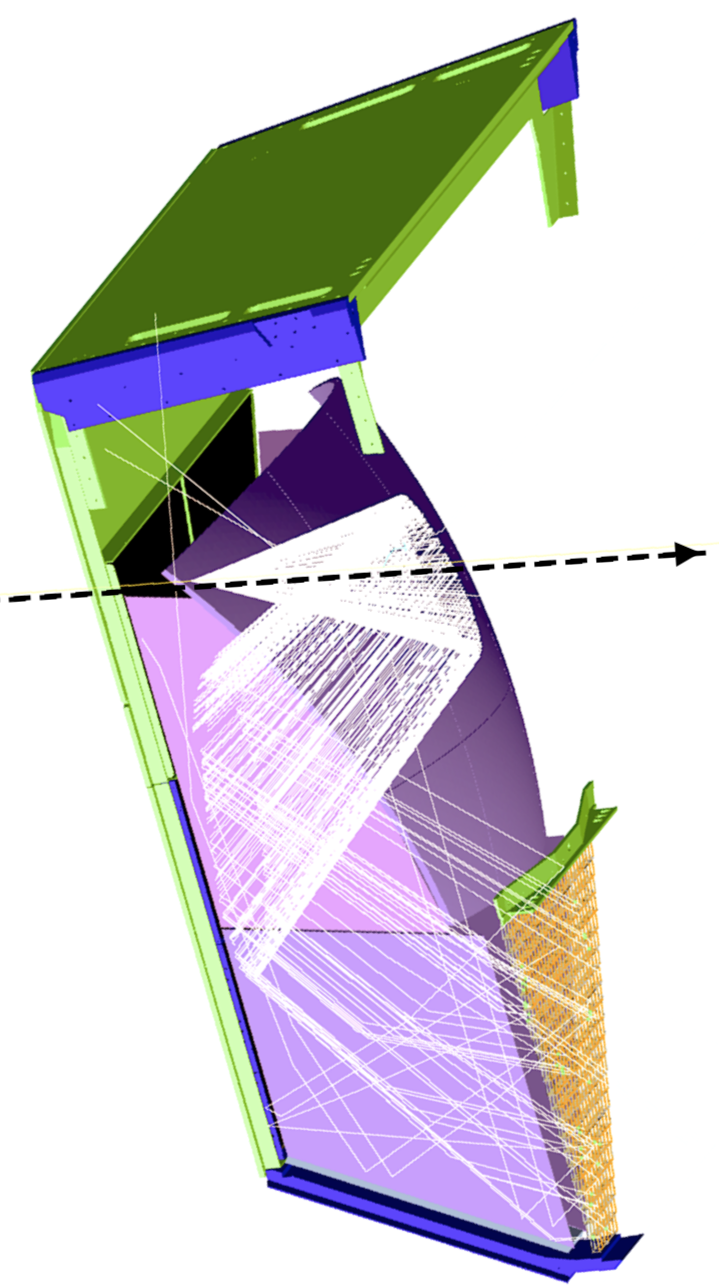
\includegraphics[width=0.99\columnwidth, keepaspectratio]{img/richGeometry.png}
	\caption{The implementation of the RICH geometry. Beam is incident from the left. A 4 GeV kaon produces a Cherenkov light cone.
			 Part of the cone reflects onto the spherical mirror and into the PMT array. The remaining photons go through the aerogel tiles
			 and bounce off the planar mirror onto the PMT array. All inefficiencies are taken into account by using the aerogel refractive index
			 and its transparency. }
	\label{fig:richGeometry}
\end{figure}

The refractive index and transparency was measured for each aerogel tile, and included in the simulation by
assigning a unique material to each aerogel volume with the proper optical properties.
Similarly for the reflectivity of each of the spherical and planar mirrors.
Theses optical properties and taken into account during the Geant4 transportation of the photons.
The quantum efficiency associated with the PMT photocathodes is taken into account in the digitization routine.

\subsubsection{Process ID}
At each Geant4 step, the local coordinates in the PMT volume are used to calculate the pixel number within that PMT.

\subsubsection{Digitization}

Photons that impinge on the PMT faces are processed with the digitization routine.
Each photon collected is input to the quantum efficiency algorithm at its wavelength to decide if it is detected.
The total number of photo-electrons is then calculated based on the PMT gains and calibrated response.
Finally, algorithms based on calibration parameters from CCDB are used to determine the leading and trailing edge times, which are
then converted to TDCs.
The digitized output bank variables are summarized in Table \ref{tab:richBank}.

\begin{table}[h]
	\begin{center}
		\begin{tabular}{| c | c | c |}
			\hline \hline
			Variable & Description                                         \\
			\hline
             sector  &                                     CLAS12 sector   \\
                pmt  &                                        PMT number   \\
              pixel  &                       pixel number within the PMT   \\
               TDCL  &                                  TDC leading edge   \\
               TDCT  &                                 TDC trailing edge   \\
               time  &                           average time of the hit   \\
               nphe  &                  number of photoelectrons arrived   \\
              npheD  &                 number of photoelectrons detected   \\
               hitn  &                                        hit number   \\
			\hline \hline
		\end{tabular}
	\end{center}
	\caption{The digitized RICH bank.}\label{tab:richBank}
\end{table}

The time window  of the RICH is set to 300 ns: all Geant4 steps within the same PMT pixel and time window are collected in one hit.
